
\section{Organización y Estructura Operacional}
\label{inicio_cap2}

Skyfilms S.A.S. cuenta con una estructura organizacional diseñada para garantizar la planificación, ejecución, supervisión y mejora continua de las operaciones con Sistemas de Aeronaves No Tripuladas (UAS), conforme a los requisitos establecidos en el Reglamento Aeronáutico de Colombia (RAC 100).

La estructura operacional se fundamenta en una cadena clara de autoridad, responsabilidades definidas y mecanismos de coordinación entre las diferentes funciones involucradas en la operación, permitiendo asegurar el cumplimiento de los requisitos técnicos, operacionales y de seguridad operacional establecidos por la Aerocivil.

La organización contempla los cargos de Gerente General, Jefe de Pilotos UAS, Gerente de Seguridad Operacional (SMS), Pilotos Remotos y Observadores, quienes desempeñan funciones específicas dentro del desarrollo de las operaciones autorizadas por Skyfilms.

\begin{tcolorbox}[colback=gray!8,colframe=black,title=Nota]

De acuerdo con la estructura organizacional actual de Skyfilms S.A.S., las funciones de Gerente General y Jefe de Pilotos UAS podrán ser desempeñadas por la misma persona. Esta asignación no limita el cumplimiento de las responsabilidades establecidas para cada cargo ni afecta la independencia funcional del Sistema de Gestión de la Seguridad Operacional (SMS).

\end{tcolorbox}

\section{Organigrama Operacional}

\begin{figure}[H]
\centering
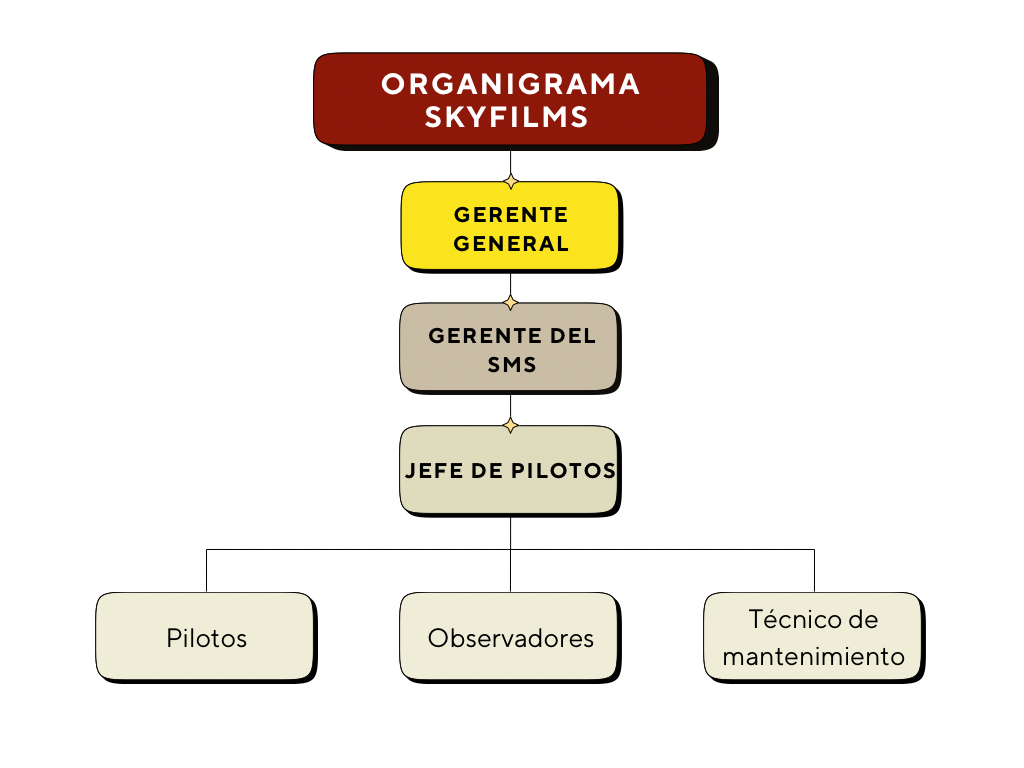
\includegraphics[width=.85\textwidth]{Imagenes/organigrama_skyfilm.PNG}
\caption{Estructura MO Skyfilms}
\end{figure}


\noindent\textbf{Nota:} La estructura organizacional presentada corresponde únicamente a la organización operacional de Skyfilms para la gestión de las operaciones UAS. Las funciones administrativas que no intervienen directamente en la operación aérea no hacen parte del presente Manual de Operaciones.

\section{Cadena de Autoridad}

La estructura de autoridad de Skyfilms S.A.S. garantiza que todas las operaciones con Sistemas de Aeronaves No Tripuladas (UAS) se desarrollen bajo una línea clara de responsabilidad, comunicación y toma de decisiones, asegurando el cumplimiento de los requisitos establecidos por la Aerocivil y por el Sistema de Gestión de la Seguridad Operacional (SMS).

La autoridad operacional se ejerce de manera jerárquica, conforme al siguiente orden:

\begin{enumerate}
    \item Gerente General.
    \item Jefe de Pilotos UAS.
    \item Pilotos Remotos.
    \item Observadores Visuales.
\end{enumerate}

El Responsable de Mantenimiento y el Gerente de Seguridad Operacional (SMS) ejercen funciones especializadas dentro de su ámbito de competencia, manteniendo independencia funcional respecto de la ejecución de las operaciones cuando así lo requiera la seguridad operacional.





\begin{table}[H]
\centering
\renewcommand{\arraystretch}{1.3}
\begin{tabularx}{\textwidth}{|p{4cm}|X|}
\hline
\textbf{Cargo} & \textbf{Nivel de autoridad} \\ \hline

Gerente General &
Máxima autoridad administrativa y operacional del explotador UAS. \\ \hline

Jefe de Pilotos UAS &
Autoriza, coordina y supervisa la ejecución de las operaciones de vuelo. \\ \hline

Gerente SMS &
Supervisa el cumplimiento de la seguridad operacional y puede recomendar la suspensión de una operación cuando identifique un riesgo no aceptable. \\ \hline

Responsable de Mantenimiento &
Autoriza la disponibilidad técnica de las aeronaves y equipos para la operación. \\ \hline

Piloto Remoto &
Responsable de la conducción segura de la aeronave durante la misión autorizada. \\ \hline

Observador Visual &
Apoya al piloto manteniendo vigilancia del entorno operacional y comunicando cualquier condición que pueda afectar la seguridad del vuelo. \\ \hline

\end{tabularx}
\caption{Cadena de autoridad operacional de Skyfilms.}
\end{table}


\section{Responsabilidades}


\subsection{Gerente General}

\subsubsection*{Objetivo del cargo}

El Gerente General es la máxima autoridad administrativa y operacional de Skyfilms S.A.S. y es responsable de garantizar que todas las operaciones con Sistemas de Aeronaves No Tripuladas (UAS) se desarrollen conforme al RAC 100, las Especificaciones Operacionales (OpSpecs), el presente Manual de Operaciones y demás normativa aplicable.

\subsubsection*{Responsabilidades}

\begin{enumerate}[label=\alph*)]
\item Aprobar el Manual de Operaciones y sus revisiones o enmiendas.
\item Garantizar la disponibilidad de recursos humanos, técnicos y financieros para la operación segura de los UAS.
\item Designar al Jefe de Pilotos UAS, al Gerente SMS y al Responsable de Mantenimiento.
\item Autorizar la incorporación de nuevas aeronaves, equipos tecnológicos y personal operativo.
\item Asegurar el cumplimiento de los requisitos establecidos por la Aerocivil.
\item Firmar las comunicaciones oficiales dirigidas a la Aerocivil.
\item Promover la cultura de seguridad operacional dentro de la organización.
\end{enumerate}

\subsubsection*{Autoridad}

El Gerente General podrá aprobar, suspender o cancelar cualquier operación cuando considere que existen condiciones que afecten la seguridad operacional, el cumplimiento normativo o los intereses de Skyfilms.

\subsubsection*{Reporta a}

No aplica.

\subsubsection*{Supervisa a}

\begin{itemize}
\item Jefe de Pilotos UAS.
\item Gerente de Seguridad Operacional (SMS).
\item Responsable de Mantenimiento.
\end{itemize}



\subsection{Jefe de Pilotos UAS}

\subsubsection*{Objetivo del cargo}

El Jefe de Pilotos UAS es el responsable de la planificación, coordinación, supervisión y control de las operaciones de vuelo desarrolladas por Skyfilms S.A.S., garantizando que todas las misiones se ejecuten de conformidad con el Reglamento Aeronáutico de Colombia (RAC 100), las Especificaciones Operacionales (OpSpecs), el presente Manual de Operaciones y demás normativa aplicable.


\subsubsection*{Responsabilidades}

Son responsabilidades del Jefe de Pilotos UAS:

\begin{enumerate}[label=\alph*)]

\item Planificar, coordinar y supervisar las operaciones UAS desarrolladas por Skyfilms.

\item Verificar que cada operación cuente con los permisos, autorizaciones y documentación exigida por la Aerocivil y demás autoridades competentes.

\item Autorizar la ejecución de las misiones de vuelo una vez verificado el cumplimiento de los requisitos operacionales, técnicos y de seguridad.

\item Asignar los pilotos remotos, observadores visuales y demás personal operativo requerido para cada misión.

\item Verificar que el personal operativo mantenga vigente su competencia, capacitación y habilitación para desempeñar sus funciones.

\item Supervisar el cumplimiento de los procedimientos establecidos en el Manual de Operaciones, Manual SMS y Manual de Control de Mantenimiento.

\item Coordinar con el Responsable de Mantenimiento la disponibilidad técnica y aeronavegabilidad de las aeronaves no tripuladas antes de cada operación.

\item Coordinar con el Gerente de Seguridad Operacional (SMS) la identificación de peligros, evaluación de riesgos y aplicación de medidas de mitigación cuando sea requerido.

\item Garantizar que los formatos operacionales, listas de chequeo, bitácoras de vuelo y demás registros sean diligenciados y archivados correctamente.

\item Supervisar el cumplimiento de los procedimientos de planificación, ejecución y cierre de las operaciones.

\item Gestionar la actualización de los registros de aeronaves, equipos tecnológicos y pilotos ante la Aerocivil cuando corresponda.

\item Participar en la investigación de incidentes, accidentes y eventos operacionales cuando sea requerido.

\item Proponer acciones de mejora para incrementar la seguridad operacional y la eficiencia de las operaciones.

\item Suspender o cancelar una operación cuando las condiciones operacionales, meteorológicas, técnicas o de seguridad no permitan garantizar un nivel aceptable de riesgo.

\end{enumerate}

\subsubsection*{Autoridad}

El Jefe de Pilotos UAS está facultado para:

\begin{itemize}

\item Autorizar el inicio de una operación UAS.

\item Suspender temporalmente una misión.

\item Cancelar una operación cuando existan condiciones inseguras.

\item Reasignar tripulaciones o aeronaves.

\item Exigir el cumplimiento de los procedimientos establecidos en el presente Manual de Operaciones.

\item Solicitar apoyo del Responsable de Mantenimiento o del Gerente SMS cuando las condiciones de la operación así lo requieran.

\end{itemize}


\textbf{Requisitos mínimos (Conforme al RAC 100.520):}
\begin{itemize}
    \item Contar con certificado vigente como Piloto UAS y capacitación en las operaciones autorizadas al explotador.
    \item Demostrar experiencia operacional de, al menos, cien (100) horas de vuelo en UAS similares a los de la flota de Skyfilms.
    \item Demostrar al menos seis (6) meses de experiencia en actividades administrativas relacionadas con operaciones en aviación no tripulada.
    \item Contar con capacitación certificada por un CIAC o CEAC de, al menos, cuarenta (40) horas en Sistema de Gestión de la Seguridad Operacional (SMS).
\end{itemize}

\subsubsection*{Reporta a}

Gerente General.

\subsubsection*{Supervisa a}

\begin{itemize}

\item Pilotos Remotos.

\item Observadores Visuales.

\end{itemize}

\begin{table}[H]
\centering
\renewcommand{\arraystretch}{1.3}
\begin{tabularx}{\textwidth}{|p{4cm}|X|}
\hline
\textbf{Cargo} & Jefe de Pilotos UAS \\ \hline
\textbf{Reporta a} & Gerente General \\ \hline
\textbf{Supervisa} & Pilotos Remotos y Observadores Visuales \\ \hline
\textbf{Autoridad} & Planificar, autorizar, supervisar, suspender y cancelar operaciones UAS. \\ \hline
\textbf{Documentos relacionados} & MO, SMS, MCM, OpSpecs y procedimientos operacionales. \\ \hline
\end{tabularx}
\caption{Resumen del cargo de Jefe de Pilotos UAS.}
\end{table}


\subsection{Gerente de Seguridad Operacional (SMS)}

\subsubsection*{Objetivo del cargo}

El Gerente de Seguridad Operacional (SMS) es el responsable de administrar, supervisar y promover el Sistema de Gestión de la Seguridad Operacional de Skyfilms S.A.S., garantizando la identificación de peligros, la gestión de riesgos y la implementación de medidas orientadas a mantener un nivel aceptable de seguridad operacional en todas las actividades relacionadas con la operación de Sistemas de Aeronaves No Tripuladas (UAS).

\subsubsection*{Responsabilidades}

Son responsabilidades del Gerente de Seguridad Operacional:

\begin{enumerate}[label=\alph*)]

\item Administrar y mantener actualizado el Sistema de Gestión de la Seguridad Operacional (SMS).

\item Identificar peligros y evaluar los riesgos asociados a las operaciones UAS.

\item Proponer e implementar medidas de mitigación para reducir los riesgos operacionales.

\item Promover la cultura de seguridad operacional dentro de la organización.

\item Realizar seguimiento a los indicadores de desempeño en seguridad operacional.

\item Gestionar el reporte voluntario y obligatorio de sucesos relacionados con la seguridad operacional.

\item Coordinar la investigación de incidentes y accidentes cuando corresponda.

\item Recomendar la suspensión de operaciones cuando identifique riesgos que superen el nivel aceptable definido por Skyfilms.

\item Verificar el cumplimiento de los procedimientos establecidos en el Manual SMS.

\item Coordinar con el Jefe de Pilotos y el Responsable de Mantenimiento la implementación de acciones correctivas y preventivas.

\item Elaborar informes periódicos sobre el desempeño del Sistema de Gestión de la Seguridad Operacional.

\end{enumerate}

\subsubsection*{Autoridad}

El Gerente de Seguridad Operacional está facultado para:

\begin{itemize}

\item Recomendar la suspensión o cancelación de una operación cuando identifique un riesgo no aceptable.

\item Solicitar la implementación inmediata de medidas de mitigación.

\item Acceder a toda la información operacional necesaria para el cumplimiento de sus funciones.

\item Solicitar investigaciones relacionadas con la seguridad operacional.

\item Presentar recomendaciones directamente al Gerente General sin necesidad de autorización previa.

\end{itemize}

\subsubsection*{Independencia funcional}

El Gerente de Seguridad Operacional ejercerá sus funciones con independencia funcional respecto de la planificación y ejecución de las operaciones UAS.

Ninguna decisión administrativa u operacional podrá limitar la presentación de reportes, recomendaciones o acciones relacionadas con la seguridad operacional.

\textbf{Requisitos mínimos (Conforme al RAC 100.520):}
\begin{itemize}
    \item Contar con un curso básico sobre SMS certificado por un CIAC o CEAC de, al menos, cuarenta (40) horas.
    \item Demostrar conocimientos o formación en áreas del sector aeronáutico.
    \item Contar con experiencia operacional aeronáutica comprobable de, al menos, doce (12) meses.
\end{itemize}

\subsubsection*{Reporta a}

Gerente General y Jefe de Piltos.

\subsubsection*{Supervisa a}

No aplica.


\begin{table}[H]
\centering
\renewcommand{\arraystretch}{1.3}

\begin{tabularx}{\textwidth}{|p{4cm}|X|}
\hline
\textbf{Cargo} & Gerente de Seguridad Operacional \\ \hline
\textbf{Reporta a} & Gerente General \\ \hline
\textbf{Supervisa} & No aplica \\ \hline
\textbf{Autoridad} & Gestionar el SMS, recomendar la suspensión de operaciones, administrar la gestión del riesgo y realizar seguimiento al desempeño de la seguridad operacional. \\ \hline
\textbf{Documentos relacionados} & Manual SMS, Manual de Operaciones, OpSpecs, procedimientos de gestión del riesgo e investigación de sucesos. \\ \hline
\end{tabularx}

\caption{Resumen del cargo de Gerente de Seguridad Operacional.}

\end{table}


\subsection{Responsable de Mantenimiento}

\subsubsection*{Objetivo del cargo}

El Responsable de Mantenimiento es el encargado de planificar, coordinar, supervisar y controlar las actividades de mantenimiento preventivo, correctivo e inspección de las aeronaves no tripuladas, baterías, estaciones de control y equipos tecnológicos utilizados por Skyfilms S.A.S., garantizando que todos los equipos se encuentren en condiciones seguras para la operación y de conformidad con el Manual de Control de Mantenimiento (MCM), las recomendaciones del fabricante y la normativa vigente.

\subsubsection*{Responsabilidades}

Son responsabilidades del Responsable de Mantenimiento:

\begin{enumerate}[label=\alph*)]

\item Elaborar y mantener actualizado el Programa de Mantenimiento de las aeronaves y equipos tecnológicos.

\item Verificar el estado de aeronavegabilidad de cada UAS antes de ser liberado para operación.

\item Ejecutar o supervisar las actividades de mantenimiento preventivo y correctivo.

\item Controlar la vida útil, ciclos de operación y estado de las baterías utilizadas por Skyfilms.

\item Mantener actualizado el historial técnico de cada aeronave, motor, batería y equipo tecnológico.

\item Garantizar que únicamente sean utilizados repuestos y componentes autorizados por el fabricante o aprobados por Skyfilms.

\item Coordinar con el Jefe de Pilotos la disponibilidad técnica de las aeronaves para las operaciones programadas.

\item Informar inmediatamente cualquier condición técnica que pueda afectar la seguridad operacional.

\item Suspender la disponibilidad operacional de cualquier aeronave que presente una condición insegura.

\item Mantener actualizados los registros de mantenimiento, inspecciones y reparaciones.

\item Verificar que las herramientas y equipos de mantenimiento se encuentren en condiciones adecuadas de uso.

\item Coordinar el envío de equipos a talleres especializados cuando las reparaciones excedan las capacidades técnicas de Skyfilms.

\end{enumerate}


\subsubsection*{Autoridad}

El Responsable de Mantenimiento está facultado para:

\begin{itemize}

\item Declarar una aeronave apta para operación.

\item Restringir o suspender la utilización de una aeronave o equipo tecnológico cuando exista una condición que afecte su aeronavegabilidad.

\item Programar inspecciones extraordinarias.

\item Solicitar mantenimiento preventivo o correctivo en cualquier momento.

\item Recomendar el retiro definitivo de equipos que no garanticen condiciones seguras de operación.

\end{itemize}


\subsubsection*{Requisitos mínimos}

El Responsable de Mantenimiento deberá:

\begin{itemize}

\item Conocer el Manual de Control de Mantenimiento (MCM).

\item Conocer las recomendaciones técnicas de los fabricantes de las aeronaves y equipos utilizados por Skyfilms.

\item Demostrar competencias en mantenimiento de sistemas UAS.

\item Mantener vigente la capacitación definida por Skyfilms para el desempeño de sus funciones.

\end{itemize}


\subsubsection*{Reporta a}

Gerente General.


\subsubsection*{Supervisa a}

Personal técnico de mantenimiento o proveedores autorizados que ejecuten actividades de mantenimiento para Skyfilms.

\begin{table}[H]
\centering
\renewcommand{\arraystretch}{1.3}

\begin{tabularx}{\textwidth}{|p{4cm}|X|}
\hline
\textbf{Cargo} & Responsable de Mantenimiento \\ \hline
\textbf{Reporta a} & Gerente General \\ \hline
\textbf{Supervisa} & Técnicos de mantenimiento o proveedores autorizados \\ \hline
\textbf{Autoridad} & Liberar, restringir o suspender la disponibilidad técnica de aeronaves y equipos. \\ \hline
\textbf{Documentos relacionados} & Manual de Control de Mantenimiento (MCM), Manual de Operaciones, Manuales del fabricante y registros técnicos. \\ \hline
\end{tabularx}

\caption{Resumen del cargo de Responsable de Mantenimiento.}

\end{table}



\subsection{Piloto Remoto UAS}

\subsubsection*{Objetivo del cargo}

El Piloto Remoto UAS es el responsable de la conducción segura de la aeronave no tripulada durante todas las fases de la operación, garantizando el cumplimiento del presente Manual de Operaciones, las Especificaciones Operacionales (OpSpecs), el Reglamento Aeronáutico de Colombia (RAC 100) y los procedimientos establecidos por Skyfilms S.A.S.


\subsubsection*{Responsabilidades}

Son responsabilidades del Piloto Remoto UAS:

\begin{enumerate}[label=\alph*)]

\item Ejecutar las operaciones de vuelo autorizadas conforme a la planificación aprobada.

\item Verificar el cumplimiento del checklist previo al vuelo antes de iniciar cualquier operación.

\item Confirmar que la aeronave, estación de control, baterías y equipos asociados se encuentren en condiciones seguras para la operación.

\item Mantener el control de la aeronave durante toda la misión.

\item Cumplir las limitaciones operacionales establecidas en las OpSpecs y en el presente Manual.

\item Mantener comunicación permanente con el Observador Visual cuando la operación así lo requiera.

\item Interrumpir o abortar la misión cuando identifique una condición que comprometa la seguridad operacional.

\item Registrar la información correspondiente en la bitácora de vuelo al finalizar cada operación.

\item Reportar cualquier incidente, accidente o condición insegura al Jefe de Pilotos y al Gerente SMS.

\item Cumplir las instrucciones emitidas por el Jefe de Pilotos y las recomendaciones de seguridad operacional emitidas por el Gerente SMS.

\end{enumerate}


\subsubsection*{Autoridad}

El Piloto Remoto está facultado para:

\begin{itemize}

\item Interrumpir inmediatamente una operación cuando identifique condiciones inseguras.

\item Declarar una situación de emergencia operacional.

\item Solicitar apoyo del Observador Visual o del Jefe de Pilotos durante la misión.

\item Negarse a iniciar una operación cuando considere que no existen condiciones seguras para realizarla.

\end{itemize}


\subsubsection*{Requisitos mínimos}

El Piloto Remoto deberá:

\begin{itemize}

\item Contar con certificado vigente como Piloto Remoto UAS conforme al RAC 100.

\item Mantener vigente la capacitación operacional establecida por Skyfilms.

\item Conocer el Manual de Operaciones, el Manual SMS y los procedimientos de emergencia.

\item Mantener la competencia operacional para el tipo de aeronave que opera.

\end{itemize}

\subsubsection*{Reporta a}

Jefe de Pilotos UAS.

\begin{table}[H]
\centering
\renewcommand{\arraystretch}{1.3}

\begin{tabularx}{\textwidth}{|p{4cm}|X|}
\hline
\textbf{Cargo} & Piloto Remoto UAS \\ \hline
\textbf{Reporta a} & Jefe de Pilotos UAS \\ \hline
\textbf{Autoridad} & Ejecutar, suspender o abortar la operación cuando la seguridad operacional lo requiera. \\ \hline
\textbf{Documentos relacionados} & Manual de Operaciones, Manual SMS, OpSpecs, listas de chequeo y procedimientos de emergencia. \\ \hline
\end{tabularx}

\caption{Resumen del cargo de Piloto Remoto UAS.}

\end{table}

\subsection{Observador Visual}

\subsubsection*{Objetivo del cargo}

El Observador Visual es el responsable de mantener vigilancia permanente sobre la aeronave no tripulada y su entorno operacional durante la ejecución de la misión, apoyando al Piloto Remoto mediante la identificación oportuna de riesgos, obstáculos, tráfico aéreo y cualquier condición que pueda afectar la seguridad operacional.

\subsubsection*{Responsabilidades}

Son responsabilidades del Observador Visual:

\begin{enumerate}[label=\alph*)]

\item Mantener contacto visual permanente con la aeronave cuando la operación así lo requiera.

\item Informar inmediatamente al Piloto Remoto sobre cualquier condición que pueda afectar la seguridad del vuelo.

\item Vigilar la presencia de personas, vehículos, obstáculos y otras aeronaves dentro del área de operación.

\item Apoyar el cumplimiento de las limitaciones operacionales establecidas para la misión.

\item Mantener comunicación efectiva con el Piloto Remoto durante toda la operación.

\item En operaciones FPV, mantener el contacto visual directo (VLOS) ininterrumpido con la aeronave para compensar la visión limitada del Piloto Remoto que utiliza las gafas FPV.

\item Colaborar en la aplicación de los procedimientos de emergencia cuando sea requerido.

\item Reportar condiciones inseguras observadas durante la operación.

\end{enumerate}

\subsubsection*{Autoridad}

El Observador Visual está facultado para:

\begin{itemize}

\item Solicitar al Piloto Remoto la interrupción inmediata de una operación cuando identifique una condición que represente un riesgo para la seguridad.

\item Recomendar modificaciones en la operación cuando observe condiciones que puedan afectar el desarrollo seguro de la misión.

\end{itemize}

\subsubsection*{Requisitos mínimos}

El Observador Visual deberá:

\begin{itemize}

\item Haber recibido la capacitación establecida por Skyfilms para el desempeño de sus funciones.

\item Conocer el presente Manual de Operaciones y los procedimientos de emergencia.

\item Mantener comunicación permanente con el Piloto Remoto durante las operaciones.

\end{itemize}


\subsubsection*{Reporta a}

Jefe de Pilotos UAS.

\begin{table}[H]
\centering
\renewcommand{\arraystretch}{1.3}

\begin{tabularx}{\textwidth}{|p{4cm}|X|}
\hline
\textbf{Cargo} & Observador Visual \\ \hline
\textbf{Reporta a} & Jefe de Pilotos UAS \\ \hline
\textbf{Autoridad} & Recomendar la interrupción de la operación cuando identifique condiciones inseguras. \\ \hline
\textbf{Documentos relacionados} & Manual de Operaciones, listas de chequeo y procedimientos de emergencia. \\ \hline
\end{tabularx}

\caption{Resumen del cargo de Observador Visual.}

\end{table}



\section{Matriz de Responsabilidades Operacionales (RACI)}

La presente matriz define la asignación de responsabilidades para los principales procesos operacionales desarrollados por Skyfilms S.A.S., permitiendo establecer de manera clara la autoridad, ejecución, consulta e información requerida para cada actividad.

Para efectos de la presente matriz se adoptan las siguientes convenciones:

\begin{itemize}
\item \textbf{R (Responsible):} Responsable directo de ejecutar la actividad.
\item \textbf{A (Accountable):} Responsable de aprobar o asumir la responsabilidad final del proceso.
\item \textbf{C (Consulted):} Debe ser consultado antes de ejecutar la actividad.
\item \textbf{I (Informed):} Debe ser informado del resultado o estado de la actividad.
\end{itemize}

\renewcommand{\arraystretch}{1.4}

\scriptsize

\begin{longtable}{|p{6.5cm}|c|c|c|c|c|c|}
\hline

\textbf{Actividad} &
\rotatebox{90}{Gerente} &
\rotatebox{90}{Jefe de Pilotos} &
\rotatebox{90}{SMS} &
\rotatebox{90}{Mantenimiento} &
\rotatebox{90}{Piloto} &
\rotatebox{90}{Observador}
\\
\hline
\endhead

Planificación de la misión &
I &
A &
C &
C &
R &
I
\\ \hline

Evaluación del riesgo operacional &
I &
C &
A/R &
C &
C &
C
\\ \hline

Autorización de la operación &
A &
R &
C &
C &
I &
I
\\ \hline

Verificación documental &
I &
A &
I &
C &
R &
I
\\ \hline

Liberación técnica del UAS &
I &
C &
I &
A/R &
I &
I
\\ \hline

Inspección preoperacional &
I &
C &
I &
C &
A/R &
R
\\ \hline

Ejecución del vuelo &
I &
I &
I &
I &
A/R &
R
\\ \hline

Gestión de emergencia &
I &
A &
C &
C &
R &
R
\\ \hline

Reporte de incidente &
I &
C &
A &
I &
R &
R
\\ \hline

Investigación de incidente &
I &
C &
A/R &
C &
C &
C
\\ \hline

Control de registros operacionales &
I &
A &
I &
I &
R &
I
\\ \hline

Control de mantenimiento &
I &
I &
I &
A/R &
C &
I
\\ \hline

Programación de mantenimiento &
I &
C &
I &
A/R &
I &
I
\\ \hline

Actualización del Manual &
A &
C/R &
C/R &
C &
I &
I
\\ \hline

Capacitación del personal &
A &
R &
C/R&
C &
I &
I
\\ \hline

\caption{Matriz RACI de responsabilidades operacionales de Skyfilms.}

\end{longtable}


\begin{tcolorbox}[title=Interpretación de la matriz]

Cuando una actividad presente simultáneamente un responsable de aprobación (A) y un responsable de ejecución (R), la actividad únicamente podrá considerarse finalizada cuando ambas responsabilidades hayan sido cumplidas.

La asignación de responsabilidades establecida en la presente matriz no exime a ningún integrante de Skyfilms del deber de informar cualquier condición que pueda afectar la seguridad operacional.

\end{tcolorbox}


\section{Sustitución temporal y delegación de funciones}

Con el fin de garantizar la continuidad de las operaciones y mantener el cumplimiento de los requisitos establecidos por el Reglamento Aeronáutico de Colombia (RAC 100), Skyfilms S.A.S. establece el presente procedimiento para la sustitución temporal de cargos y la delegación de funciones cuando un responsable no pueda ejercer sus funciones por ausencia, incapacidad, vacaciones, comisión de servicio o cualquier otra circunstancia que impida el normal desarrollo de sus actividades.

La delegación de funciones no exime al titular del cargo de las responsabilidades que le correspondan cuando reasuma sus funciones, ni modifica las responsabilidades asignadas a los demás integrantes de la organización.


\subsection*{Principios generales}

La sustitución temporal de cargos se regirá por los siguientes principios:

\begin{enumerate}[label=\alph*)]

\item La continuidad operacional no deberá verse afectada por la ausencia temporal de un responsable.

\item Ninguna persona podrá asumir funciones para las cuales no haya sido previamente designada y demostrada su competencia.

\item La delegación deberá quedar documentada cuando implique decisiones operacionales o administrativas relevantes.

\item Las funciones relacionadas con la seguridad operacional conservarán la independencia funcional establecida en el Sistema de Gestión de la Seguridad Operacional (SMS).

\end{enumerate}

\renewcommand{\arraystretch}{1.4}

\begin{longtable}{|p{4cm}|p{5cm}|p{5cm}|}

\hline

\textbf{Cargo} &
\textbf{Sustituto temporal} &
\textbf{Condición para asumir el cargo}

\\ \hline

Gerente General &
Jefe de Pilotos UAS &
Cuando exista delegación expresa del Gerente General.

\\ \hline

Jefe de Pilotos UAS &
Piloto Remoto designado por la Gerencia &
Debe cumplir los requisitos establecidos para el cargo y ser designado formalmente.

\\ \hline

Gerente SMS &
Profesional designado por la Gerencia con competencias en SMS &
Debe conservar la independencia funcional respecto de la operación.

\\ \hline

Responsable de Mantenimiento &
Técnico competente o proveedor autorizado &
Debe demostrar competencia para ejecutar las actividades delegadas.

\\ \hline

Piloto Remoto &
Otro Piloto Remoto habilitado &
Debe encontrarse vigente y autorizado para operar el tipo de aeronave correspondiente.

\\ \hline

Observador Visual &
Otro Observador Visual capacitado &
Debe haber recibido la capacitación establecida por Skyfilms.

\\ \hline

\caption{Sustitución temporal de cargos operacionales.}

\end{longtable}


\subsection*{Ejercicio simultáneo de cargos}

Durante la etapa inicial de operación de Skyfilms S.A.S., una misma persona podrá ejercer simultáneamente los cargos de Gerente General y Jefe de Pilotos UAS, siempre que:

\begin{enumerate}[label=\alph*)]

\item Se garantice el cumplimiento integral de las responsabilidades asignadas a ambos cargos.

\item No se comprometa la seguridad operacional.

\item Se mantenga la independencia funcional del Gerente de Seguridad Operacional (SMS).

\item Se conserve la adecuada supervisión de las actividades de mantenimiento.

\end{enumerate}


\subsection*{Delegación de autoridad}

Cuando un responsable delegue temporalmente sus funciones deberá garantizar, como mínimo:

\begin{itemize}

\item La entrega de la información necesaria para la continuidad de las operaciones.

\item La comunicación al personal involucrado.

\item La actualización de los registros correspondientes.

\item La conservación de la trazabilidad documental de la delegación.

\end{itemize}


\section{Coordinación entre las áreas operacionales}

Con el fin de garantizar la ejecución segura, eficiente y conforme a la reglamentación vigente de todas las operaciones UAS, Skyfilms establece mecanismos permanentes de coordinación entre las áreas de Operaciones, Seguridad Operacional (SMS), Mantenimiento y Gerencia General.

La coordinación entre las diferentes áreas se desarrolla durante todas las fases de la operación, desde la planificación de la misión hasta el cierre documental de la misma.



\renewcommand{\arraystretch}{1.4}

\begin{longtable}{|p{4cm}|p{5cm}|p{6cm}|}

\hline

\textbf{Área} &
\textbf{Coordina con} &
\textbf{Objeto de la coordinación}

\\ \hline

Gerencia General &
Todas las áreas &
Disponibilidad de recursos, aprobación de políticas y toma de decisiones estratégicas.

\\ \hline

Jefe de Pilotos &
SMS y Mantenimiento &
Planificación de operaciones, disponibilidad técnica, gestión del riesgo y asignación de tripulaciones.

\\ \hline

SMS &
Operaciones y Mantenimiento &
Identificación de peligros, mitigación de riesgos, investigación de incidentes y seguimiento de acciones correctivas.

\\ \hline

Mantenimiento &
Operaciones &
Disponibilidad técnica de aeronaves, inspecciones, mantenimiento preventivo y correctivo.

\\ \hline

Piloto Remoto &
Observador Visual &
Ejecución segura de la misión, comunicaciones y aplicación de procedimientos de emergencia.

\\ \hline

\caption{Coordinación entre las áreas operacionales de Skyfilms.}

\end{longtable}



















\section{Sistema y Procedimiento para el Control y Supervisión de las Operaciones UAS}

Skyfilms implementa un sistema de control y supervisión basado en la estandarización de procedimientos, el uso de listas de verificación operacionales y la designación clara de responsables en cada fase de la operación. Este sistema asegura que todas las misiones se ejecuten de conformidad con el Manual de Operaciones y las disposiciones establecidas por la Aerocivil.

\subsection*{Control de las operaciones}
El control de las operaciones se realiza a través de los siguientes elementos:
\begin{itemize}
    \item Diligenciamiento obligatorio de formatos de solicitud y autorización de vuelo, conforme a los requisitos de la Aerocivil.
    \item Aplicación de listas de verificación de pre-vuelo, vuelo y post-vuelo, supervisadas por el Jefe de Pilotos.
    \item Registro de horas de vuelo, aeronaves utilizadas, pilotos responsables y observadores asignados en la bitácora oficial de Skyfilms.
    \item Reporte inmediato de incidentes, anomalías o desviaciones operacionales al Gerente de Seguridad Operacional.
\end{itemize}

\subsection*{Supervisión de las operaciones}
La supervisión se articula a través de las siguientes responsabilidades:
\begin{itemize}
    \item El \textbf{Jefe de Pilotos} supervisa la correcta ejecución de cada operación, revisando planes de vuelo, asignación de recursos y cumplimiento de checklists.
    \item El \textbf{Gerente de Seguridad Operacional} monitorea el cumplimiento de las normas de seguridad operacional, analiza reportes de incidentes y propone medidas de mitigación.
    \item El \textbf{Gerente General} garantiza que los informes de supervisión sean presentados ante la Aerocivil cuando así se requiera.
\end{itemize}

\subsection*{Procedimiento}
El procedimiento para el control y la supervisión de las operaciones se desarrolla de la siguiente manera:
\begin{enumerate}
    \item El piloto presenta la solicitud de operación al Jefe de Pilotos con la información requerida.
    \item El Jefe de Pilotos valida la documentación, aprueba la operación y designa tripulación y recursos.
    \item Durante el vuelo, el piloto y observador/es siguen las listas de verificación operacionales, bajo la supervisión directa del Jefe de Pilotos.
    \item Al finalizar la operación, el piloto completa el registro de vuelo y el Técnico UAS realiza la inspección post-vuelo de la aeronave.
    \item El Gerente de Seguridad Operacional revisa los reportes de cada misión, consolida hallazgos y los comunica al Gerente General.
    \item En caso de incidentes, el Gerente de Seguridad Operacional inicia el proceso de análisis y emite las recomendaciones correspondientes.
\end{enumerate}



\section{Integración del Sistema de Gestión Operacional}

La estructura organizacional definida en el presente capítulo constituye la base del Sistema de Gestión Operacional de Skyfilms S.A.S.

Las funciones, responsabilidades, competencias y mecanismos de coordinación establecidos para cada cargo se complementan con los procedimientos operacionales, el Sistema de Gestión de la Seguridad Operacional (SMS), el Manual de Control de Mantenimiento (MCM), las Especificaciones Operacionales (OpSpecs) y los formatos controlados de la organización.

El control y supervisión de las operaciones UAS se ejerce mediante:

\begin{itemize}

\item La estructura organizacional.

\item La cadena de autoridad.

\item La Matriz RACI.

\item Los procedimientos operacionales.

\item Las listas de chequeo.

\item Los registros de vuelo.

\item Los procesos de mantenimiento.

\item El Sistema de Gestión de la Seguridad Operacional.

\end{itemize}

\section{Instalaciones Administrativas y Operativas}
La sede administrativa y de coordinación de operaciones de Skyfilms S.A.S. se encuentra ubicada en la ciudad de Ibagué, Tolima, desde donde se centraliza la planificación de los vuelos, el control documental, el resguardo de la biblioteca técnica y la gestión de la seguridad operacional (SMS).

Debido a la naturaleza de la producción audiovisual, Skyfilms no opera desde bases fijas de lanzamiento. Las zonas de operación (Dronpuertos) son de carácter móvil y temporal, estableciéndose en los lugares de rodaje específicos de acuerdo con la planificación de cada misión, los permisos obtenidos y las condiciones de seguridad estipuladas en el presente manual. El almacenamiento de las aeronaves y baterías se realiza en la base principal bajo condiciones controladas de temperatura y humedad, aisladas de personal no autorizado.
